\begin{figure}
\begin{tabular}{cc}
\begin{subfigure}[b]{0.45\textwidth}
\begin{center}
{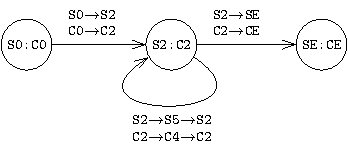
\includegraphics[scale=1.1]{chapters/figures/figSumListProductCfg.pdf}}
\end{center}
\caption{\label{fig:llTraverseProduct}Product-CFG}
\end{subfigure}%
&
\begin{subfigure}[b]{0.55\textwidth}
\begin{center}
\begin{footnotesize}
\begin{tabular}{|c|l|}
\hline
\tt PC-Pair & \multicolumn{1}{c|} {\tt Invariants} \\
\hline
\hline
${\tt (S0:C0)}$ &
\Tstrut ${\tt {\circled{P}}\  l_{S}\indEq{}Clist^{lnode}_{m}(l_{C})}$ \\
\multirow{2}{*}{${\tt (S2:C2)}$} &
\Tstrut \Bstrut ${\tt {\scriptsize \circled{I1}}\  l_{S}\indEq{}Clist^{lnode}_{m}(l_{C})}$ \\ & ${\tt {\scriptsize \circled{I2}}\  sum_{S}=sum_{C}}$ \\
${\tt (SE:CE)}$ &
\Tstrut \Bstrut ${\tt {\circled{E}}\  ret_{S}=ret_{C}}$ \\
\hline
\end{tabular}
\end{footnotesize}
\vspace{13px}
\end{center}
\caption{\label{fig:llTraverseProductInv}Node Invariants of the Product-CFG}
\end{subfigure}%
\\
\end{tabular}
\caption{\label{fig:llTraverseProductCFGInvs} Product-CFG between the IRs in \cref{fig:llTraverseSpec,fig:llTraverseC}. The inductive invariants of the Product-CFG are given in \cref{fig:llTraverseProductInv}.}
\end{figure}
